\documentclass[11pt, letterpaper]{article}
\usepackage[margin=1in]{geometry}
\usepackage{amsmath}
\usepackage{enumitem}
\usepackage{amsfonts}
\usepackage{siunitx}
\usepackage{graphicx}
\usepackage{booktabs}

\title{EMCH 290 Quiz \#6 Solution}
\author{Solved by Jacob C. Vaught}
\date{Fall 2023}

\begin{document}

\maketitle

\section*{Problem \#1}
\subsection*{Problem 1a: Isentropic Process}
\textbf{Question:} What is an isentropic process?
\newline\textbf{Answer:} An isentropic process is an idealization in which the process is both adiabatic and reversible. This means that there is no heat transfer with the surroundings (\( Q=0 \)) and no entropy generation within the system (\( \sigma=0 \)), hence the entropy remains constant (\( \Delta S=0 \)).

\subsection*{Problem 1b: Internally Reversible Process}
\textbf{Question:} In the limit, is it possible for a process of a closed system to be internally reversible, but there could be irreversibilities within the surroundings? Provide an example.
\newline\textbf{Answer:} Yes, it is possible. An example would be a perfectly insulated system that expands against a piston in such a way that the expansion is quasi-static, meaning there are no internal irreversibilities. However, if the piston pushes against the surroundings causing, for instance, a stirring of an external fluid, this could introduce irreversibilities outside the system.

\subsection*{Problem 1c: Closed System Process}
\textbf{Question:} A closed system undergoes a process for which \( S2 = S1 \). Must the process be internally reversible? Explain.
\newline\textbf{Answer:} Not necessarily. While \( S2 = S1 \) indicates that the total entropy of the system has not changed, it does not account for entropy that could have been generated within the system and then transferred out. The process is only internally reversible if there is no entropy generation (\( \sigma=0 \)).

\subsection*{Problem 1d: Entropy at Exit and Inlet}
\textbf{Question:} For a one-inlet, one-exit control volume at steady state, the specific entropy at the exit must \_\_\_\_\_\_\_\_\_\_\_\_ (than) the specific entropy at the inlet if there is no heat transfer.
\newline\textbf{Answer:} For a one-inlet, one-exit control volume at steady state with no heat transfer, the specific entropy at the exit must be \textbf{greater than or equal to} the specific entropy at the inlet. This is due to the possibility of entropy generation within the control volume.

\subsection*{Problem 1e: h–s Diagram}
\textbf{Question:} The h–s diagram is commonly known as the \_\_\_\_\_\_\_\_\_\_\_\_ diagram.
\newline\textbf{Answer:} The h–s diagram is commonly known as the \textbf{Mollier} diagram.

\subsection*{Problem 1f: Entropy Balance for SISO System}
Identify the underlined components of the following equation and rewrite it for a SISO (Single Input, Single Output) system.
\[ \frac{dS_{cv}}{dt} = \sum_j \frac{\dot{Q}_j}{T_j} + \sum_i \dot{m}_i s_i - \sum_e \dot{m}_e s_e + \dot{\sigma}_{cv} \]

\textbf{Solution:}
For a Single Input, Single Output system, the equation simplifies to:
\[ \frac{dS_{cv}}{dt} = \frac{\dot{Q}}{T} + \dot{m}_i s_i - \dot{m}_e s_e + \dot{\sigma}_{cv} \]

\textbf{Definitions}
\begin{itemize}
    \item \( \frac{dS_{cv}}{dt} \): Rate of change of entropy within the control volume for a SISO system.
    \item \( \frac{\dot{Q}}{T} \): Entropy transfer for the single heat transfer process occurring across the control boundary, divided by the temperature at the boundary.
    \item \( \dot{m}_i s_i \): Rate of entropy flow associated with the single mass flow entering the control volume.
    \item \( \dot{m}_e s_e \): Rate of entropy flow associated with the single mass flow leaving the control volume.
    \item \( \dot{\sigma}_{cv} \): Rate of entropy generation within the control volume for a SISO system.
\end{itemize}

\newpage
\section*{Problem \#2}
One kilogram of water contained in a piston–cylinder assembly, initially at \( 160^\circ C \), \( 150 \, kPa \), undergoes an isothermal compression process to saturated liquid. For the process, \( W = -475.1 \, \si{\kilo\joule} \). Determine for the process,

\begin{enumerate}[label=\alph*.]
    \item the heat transfer, in \si{\kilo\joule},
    \item the change in entropy, in \si{\kilo\joule\per\kelvin}.
    \item Show the process on a sketch of the \( T-s \) diagram.
\end{enumerate}

\section*{Analysis}

\textbf{(a)} We know that \( \Delta U + \Delta KE + \Delta PE = Q - W \)

Since \( \Delta KE \) and \( \Delta PE \) are negligible, we have:

\[ Q = W + \Delta U = W + m(u_2 - u_1) \]

From the steam tables, we find:

\[ u_1 = 2595.2 \, \si{\kilo\joule\per\kilogram} \quad \text{(from Table A-4)} \]
\[ u_2 = 674.86 \, \si{\kilo\joule\per\kilogram} \quad \text{(from Table A-2)} \]


Substituting the values, we get:

\[ Q = -475.1 \, \si{\kilo\joule} + 1 \, \si{\kilogram}(674.86 - 2595.2) \, \si{\kilo\joule\per\kilogram} \]

\[ Q = -2395.44 \, \si{\kilo\joule} \]
\newline
\textbf{(b)} The entropy change \( \Delta S \) is given by:

\[ \Delta S = m(s_2 - s_1) \]

Again from the steam tables:
\[ s_1 = 7.74665 \, \si{\kilo\joule\per\kilogram\per\kelvin} \quad \text{(from Table A-4)} \]
\[ s_2 = 1.9427 \, \si{\kilo\joule\per\kilogram\per\kelvin} \quad \text{(from Table A-2)} \]

So, the change in entropy is:

\[ \Delta S = 1 \, \si{\kilogram}(1.9427 - 7.74665) \, \si{\kilo\joule\per\kilogram\per\kelvin} \]

\[ \Delta S = -5.80395 \, \si{\kilo\joule\per\kelvin} \]
\newpage

\textbf{(c)} T-s Diagram

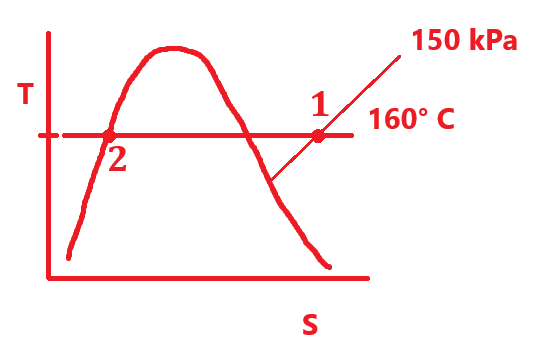
\includegraphics[width=0.8\textwidth]{T-s_Diagram_615.png}

\newpage
\section*{Problem \#3}
Five kg of water contained in a piston–cylinder assembly expand from an initial state where \( T_1 = 400^\circ C \), \( p_1 = 700 \, kPa \) to a final state where \( T_2 = 200^\circ C \), \( p_2 = 300 \, kPa \), with no significant effects of kinetic and potential energy. It is claimed that the water undergoes an adiabatic 
process between these states while developing work. Evaluate 
this claim.
\newline\newline
The table below summarizes the properties of water at the initial and final states:

\begin{table}[h]
\centering
\begin{tabular}{@{}ccccccc@{}}
\toprule
State & \( T \, (^\circ C) \) & \( p \, (kPa) \) & \( v \, (m^3/kg) \) & \( u \, (kJ/kg) \) & \( h \, (kJ/kg) \) & \( s \, (kJ/kg \cdot K) \) \\ \midrule
1     & 400                   & 700               & 0.4397             & 2960.9            & 3268.7           & 7.6350                    \\
2     & 200                   & 300               & 0.7160             & 2650.7            & 2865.5           & 7.3115                    \\ \bottomrule
\end{tabular}
\caption{Thermodynamic properties of water at states 1 and 2.}
\end{table}
\section*{Analysis}
The entropy change for the process is calculated as follows:
\begin{align*}
\Delta S &= S_2 - S_1 \\
\Delta S &= 7.3115 \, \text{kJ/kg} \cdot K - 7.6350 \, \text{kJ/kg} \cdot K \\
\Delta S &= -0.3235 \, \text{kJ/kg} \cdot K
\end{align*}
\newline
For the mass of water, the total entropy change \( \sigma \) is:
\begin{align*}
\sigma &= m \cdot \Delta S \\
\sigma &= 5 \, \text{kg} \cdot (-0.3235 \, \text{kJ/kg} \cdot K) \\
\sigma &= -1.6175 \, \text{kJ/K}
\end{align*}

Since \( \sigma \) is not equal to zero, the claim that the water undergoes an adiabatic process is false as there is an entropy decrease, indicating heat transfer out of the system.
\end{document}
